\documentclass[]{beamer}

\usepackage{lipsum}
\usepackage{pgfpages}
\usepackage{graphics}

\graphicspath{{img/}}

\mode<handout>{%
%	\setbeameroption{show notes}
}

\usetheme{AnnArbor}
\usecolortheme{beaver}

\begin{document}
	\title[Actieherkenning met de Kinect sensor]{Live actieherkenning met skeletdata van de Kinect Sensor}
	\date{}
	\frame{\titlepage}
	\begin{frame}
		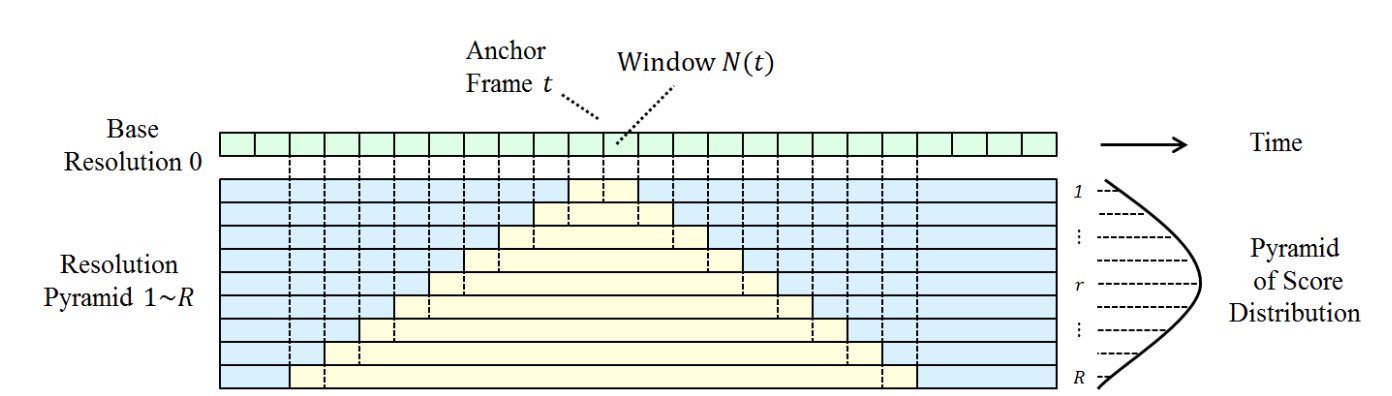
\includegraphics[width=\textwidth]{pyramid}
	\end{frame}
	\begin{frame}
		\frametitle{Voorstel}

		
		\begin{itemize}
			\item Gebruik maken van meerdere resoluties \cite{Yang2012},
			\item en aangepaste vorm van Cov3DJ \cite{Hussein2013}
		\end{itemize}

	\end{frame}
	\begin{frame}
	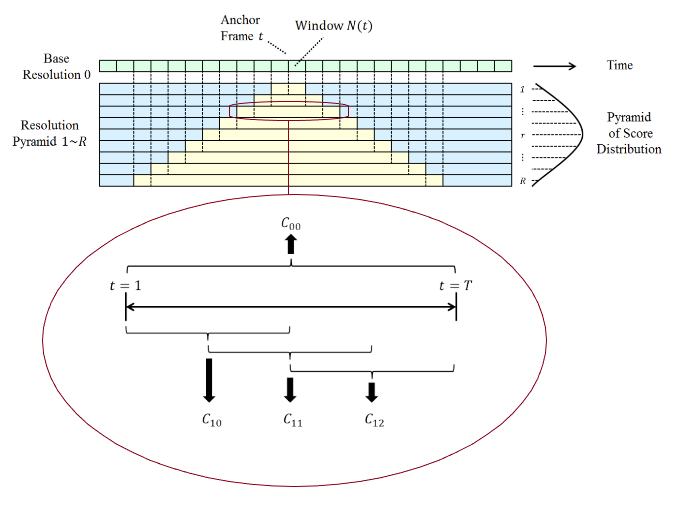
\includegraphics[width=\textwidth]{voorstel}
	\end{frame}

	\begin{frame}
		\frametitle{Datasets}
		\begin{itemize}
			\item MSRC-12 Kinect
			\item UTKinect
		\end{itemize}
	\end{frame}

	\begin{frame}[allowframebreaks]
		\frametitle{Referenties}
		\bibliographystyle{ieeetr}
		\bibliography{../../thesis/bib/library.bib}
	\end{frame}
	

\end{document}